\section{Analisi esplorativa}
\subsection{Descrizione del dataset}
Il dataset si compone di 13611 istanze, ognuna rappresentante un fagiolo
differente.
Sono presenti 16 feature, di cui 14 a valore continuo e 2 a valore intero.
4 di esse sono fattori di forma, mentre
le rimanenti 12 sono legate alla dimensione del fagiolo e alle
sue proporzioni.
Non sono presenti istanze con valori mancanti, e non è quindi necessario
adottare alcuna misura per gestire questo caso eccezionale.

Per quanto riguarda il target, invece, a ogni istanza è associata una label,
che corrisponde al nome della varietà a cui
essa appartiene. Per evitare di trattare label sottoforma di stringhe,
esse vengono tradotte, tramite label encoding, in interi maggiori o uguali a 0.
Il mapping che si ottiene è il seguente: Barbunya $\rightarrow$ 0, 
Bombay $\rightarrow$ 1, Cali $\rightarrow$ 2, Dermason $\rightarrow$ 3,
Horoz $\rightarrow$ 4, Seker $\rightarrow$ 5, Sira $\rightarrow$ 6.

Il dataset è fortemente sbilanciato, soprattutto le classi 3 e 5, che
presentano una differenza di 3000 istanze. 
\begin{Figure}
    \centering
    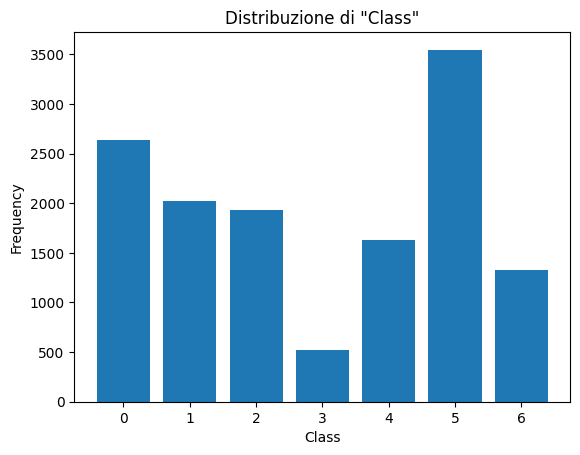
\includegraphics[width=\linewidth]{img/unbalanced_dataset.png}
    \captionof{figure}{Numero di istanze per classe.}
\end{Figure}
Per questo motivo non sarà possibile
utilizzare metriche di performance che non tengono conto di diversi costi
di errore per le classi, come l'accuratezza e la ROC-AUC, ma sarà necessario adottare misure
come la precisione, il richiamo, o l'f1-score (che corrisponde alla media
armonica tra precisione e richiamo).
Dovendo assegnare a tutte le classi la stessa importanza, inoltre, dovranno essere
preferite misure di macro-performance a quelle di micro-performance.

\subsection{Dimensionality reduction}
Ridurre la dimensionalità dello spazio delle istanze permette di ridurre la
complessità dei modelli e la probabilità di un loro eventuale overfitting.
La dimensionality reduction può essere effettuata rimuovendo feature superflue
e/o tramite PCA.

Il valore assunto da una feature dovrebbe idealmente dipendere solo
da fattori legati al dominio in cui si sta operando, e non al modo con cui 
si interagisce con il dominio stesso. 
In questo caso, però, 4 feature non dipendono esclusivamente dalla varietà a cui
il fagiolo appartiene, ma anche dalla distanza a cui esso è stato
inquadrato nella prima fase di Computer Vision. Queste 4 feature sono: 
Area, ovvero il numero di pixel occupati dal fagiolo; ConvexArea, ovvero il
numero di pixel occupati dalla più piccola figura convessa che racchiude
il fagiolo; MajorAxisLength, ovvero la lunghezza dell'asse maggiore dell'ellisse
con cui il fagiolo viene approssimato; MinorAxisLength, ovvero la lunghezza
dell'asse minore dell'ellisse che approssima il fagiolo.
Rimuovere semplicemente queste feature porterebbe, però, a un'importante perdita
di informazioni. Si può notare che i rapporti tra ConvexArea e Area
e tra MajorAxisLength e MinorAxisLength rimangono costanti al variare della
distanza di inquadratura, e posso essere utilizzati per caratterizzare una
varietà.
Ma questi rapporti sono già espressi da altre due feature del dataset,
rispettivamente Extent e AspectRatio, e quindi tutte e quattro le feature
citate possono essere rimosse, senza alcuna perdita di informazioni.

Una conseguenza molto importante della rimozione di queste feature è che le
due feature intere, Area e ConvexArea, non sono più presenti, rimanendo quindi con sole
feature continue: questo permetterà di applicare lo scaling e PCA a tutte le
feature e di usare il Gaussian Naive Bayes classifier senza preoccuparsi di
gestire le feature intere.

L'altra tecnica di dimensionality reduction che è possibile applicare è
la Principal Component Analysis, utile quando le feature sono fortemente correlate.
Prima ancora di effettuare la PCA, però, è necessario suddividere il dataset
in istanze di addestramento e istanze di test. La PCA verrà applicata, o per meglio
dire i coefficienti verranno calcolati, sulle sole istanze dedicate 
al training, mantenendo così una totale indipendenza tra istanze di addestramento
e istanze di test.
Essendo il dataset composto da una quantità medio-alta di istanze,
esso può essere suddiviso in
modo tale che le istanze di test coprano una percentuale tra il 20\% e 
il 40\% dell'intero dataset.
In questo caso, si è scelto di riservare il 25\% di istanze per il testing,
ottenendo, di conseguenza, 10208 istanze di addestramento e 3403 istanze di test.

Una volta effettuato lo splitting del dataset, è quindi possibile applicare la PCA.
Prima di farlo è però necessario effettuare lo scaling di tutte
le feature: la PCA, infatti, sceglie le componenti principali in base alla
loro varianza e feature con un'ampia scala, solitamente dotate di una 
varianza maggiore, potrebbero influenzare maggiormente la varianza delle
componenti principali e portare a una scelta artificiosa.
Lo scaling di una feature prevede di modificare tutti i suoi valori in modo 
che la sua media sia 0 e la sua varianza sia 1.

Il 95\% della varianza di questo dataset può essere espresso usando solo
5 componenti principali: il numero di feature si è quindi ridotto da 12 a 5.

\begin{Figure}
    \centering
    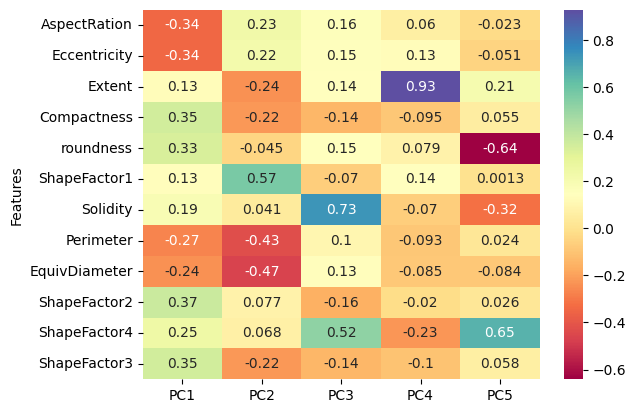
\includegraphics[width=\linewidth]{img/pca_features_weights.png}
    \captionof{figure}{Pesi delle feature per ogni componente principale.}
\end{Figure}

D'ora in poi, quando si parlerà di istanze di addestramento si farà riferimento
alle istanze di addestramento a cui è già stata applicata la PCA.
Si ricorda anche che, prima di poter utilizzare le istanze di test per verificare
le performance del modello, è necessario trasformarle usando lo stesso
scaler e le stesse componenti principali calcolati sulle istanze di addestramento. 
